\RequirePackage[hyphens]{url}
\documentclass[12pt,a4paper]{article}
\usepackage[left=2cm, right=2cm, top=2cm, bottom=2cm]{geometry}

\setlength{\parindent}{1cm}
\setlength{\parskip}{0.5em}
\renewcommand{\baselinestretch}{1.5}

\usepackage{array}
\newcolumntype{C}[1]{>{\centering\let\newline\\\arraybackslash\hspace{0pt}}m{#1}}

\newcommand\tab[1][1cm]{\hspace*{#1}}

\usepackage[utf8]{vietnam}
\usepackage[utf8]{inputenc}
\usepackage{xpatch}
\usepackage{amsmath,array,url}
\usepackage{amssymb}
\usepackage{amsfonts}
\usepackage{extarrows}
\usepackage{graphicx}
\graphicspath{ {img/} }

\usepackage{enumitem}
\usepackage{tcolorbox}
\usepackage{multirow}
\usepackage{hyperref}
\hypersetup{
	colorlinks=true,
	linkcolor=black,
	urlcolor=black,
}
\urlstyle{same}
\usepackage{listings}

\makeatletter
\newcommand{\mtmathitem}{%
\xpatchcmd{\item}{\@inmatherr\item}{\relax\ifmmode$\fi}{}{\errmessage{Patching of \noexpand\item failed}}
\xapptocmd{\@item}{$}{}{\errmessage{appending to \noexpand\@item failed}}}
\makeatother

\newenvironment{mathitem}[1][]{%
\itemize[#1]\mtmathitem}{$\endlist}                    %$

\newenvironment{mathenum}[1][]{%
\enumerate[#1]\mtmathitem}{$\endlist}                  %$

\newenvironment{mathdesc}[1][]{%
\description[#1]\mtmathitem}{$\endlist}                %$

\title{\vspace{-1.5cm}Báo cáo bài tập lớn môn Xử lý ảnh\\Nhận diện chữ monospace trong ảnh chụp}
\author{Nhóm 18* - lớp INT3404 1}
\date{Học kỳ 1, 2020}

\begin{document}

\maketitle

\textbf{Thành viên trong nhóm:}
\begin{itemize}
	\item Nguyễn Cẩm Tú - 18020058
	\item Hoàng Minh Đức Anh - 18020003
\end{itemize}

\textbf{Link repo code:} \url{https://github.com/tunc2112/uet-img-processing}

\textit{\* Nhóm đăng ký thuyết trình}

\pagebreak

\tableofcontents

\pagebreak

\section{Mở đầu}

\indent Trong những năm gần đây, với sự gia tăng ngày càng mạnh số lượng học sinh, sinh viên học lập trình, các hội nhóm, diễn đàn lập trình ngày càng nhiều. Mỗi ngày, có hàng chục, hàng trăm lượt hỏi của người học lập trình trên khắp các hội nhóm, diễn đàn lớn nhỏ, mà phần lớn trong số này là các câu hỏi về gỡ lỗi code. Để người khác có thể giúp đỡ, người hỏi cần cung cấp source code và error log (nếu có), tuy nhiên có rất nhiều người hỏi không cung cấp source code dưới dạng text, thay vào đó là hình chụp màn hình soạn thảo code của mình. Hình chụp có thể được chụp bằng chức năng chụp màn hình có sẵn do phần mềm trên máy tính hỗ trợ, thậm chí có thể được chụp qua camera điện thoại hoặc máy ảnh. Do vậy, để giảm thiểu lượng hình ảnh chụp source code cũng như giúp đỡ những người khác không mất công gõ lại code, nhóm chúng tôi lựa chọn đề tài áp dụng một số thư viện OCR hỗ trợ cho ngôn ngữ Python để chuyển đổi ảnh chụp sang dạng text.

Các tool chuyển đổi online (như www.onlineocr.net/) không đảm bảo toàn vẹn nội dung source code, không kể sai sót khi không nhận diện đúng kí tự, kết quả còn làm mất kí tự tab đầu dòng. Mục tiêu của chúng tôi là cố gắng khắc phục các nhược điểm trên, sau quá trình chuyển đổi, đoạn văn bản sẽ có đủ kí tự, nhất là kí tự whitespace nhất có thể.

\section{Phương pháp tiếp cận}

Khi soạn thảo source code, người ta thường soạn thảo trên nền IDE hoặc một text editor nào đó. Giao diện của một IDE thường có:

\begin{itemize}
	\item Khu vực soạn thảo
	\item Project view
	\item Error view
	\item Menubar
\end{itemize}

Các IDE thường có viền lớn ngăn cách giữa các phần (ví dụ: left side và editor side, editor side và error log). Thông thường, khu vực soạn thảo có thể có cả line count. Những dữ liệu dạng text từ những vùng không phải khu vực soạn thảo sẽ làm "nhiễu" thông tin, làm sai lệch dữ liệu ta mong muốn thu được. Như vậy, việc cắt ảnh để chỉ giữ lại khu vực soạn thảo là cần thiết.

\subsection{Các bước thực hiện}

\begin{enumerate}
	\item Lọc nhiễu ảnh.

	\item Từ 1 ảnh lớn, cắt bỏ những phần không nằm thuộc khu vực soạn thảo (menubar, terminal panel,...):\begin{itemize}
		\item Dùng (Canny và) Hough Line Transform để xác định các đường thẳng là đường viền giữa các phần.
		\item Từ những đường thẳng thu được, thực hiện cắt ảnh. Ta cần phải lựa chọn đường thẳng nào áp dụng vào việc cắt để tránh mất mát thông tin.
	\end{itemize}
	\item Áp dụng thư viện opencv và 1 thư viện OCR, nhận dạng chữ và trích xuất dưới dạng text.

	\item So sánh độ chính xác của đoạn text kết quả so với output mẫu.
\end{enumerate}

\subsection{Yêu cầu hệ thống tối thiểu}

\begin{itemize}
	\item python3.6+
	\item Thư viện: opencv, numpy, Pillow, scipy.
	\item \href{https://github.com/madmaze/pytesseract}{pytesseract}
	\item \href{https://gitlab.gnome.org/World/OpenPaperwork/pyocr}{pyocr}
	\item \href{https://github.com/sirfz/tesserocr}{tesserocr}
\end{itemize}

3 thư viện OCR trên đây không chỉ dùng thư viện opencv để đọc ảnh mà còn dùng thư viện Pillow.

\section{Thực hiện chi tiết}

\subsection{Thu thập dữ liệu}

\indent Tập dữ liệu ban đầu là ảnh chụp màn hình các loại, bao gồm 122 ảnh đặt trong thư mục img\_src, bao gồm:

\begin{itemize}
	\item 109 ảnh chụp qua chức năng PrintScreen (gọi là ảnh loại (1)), mã số ảnh từ 001 đến 114.
	\item 13 ảnh chụp qua máy ảnh ngoài (gọi là ảnh loại (2)), mã số ảnh từ 201 đến 213.
\end{itemize}

Định dạng tên của file ảnh là "src<mã số ảnh>.(png|jpg|jpeg)".

Từ dữ liệu được lấy ra từ các ảnh, tạo output mẫu là các file text được đặt trong thư mục expected\_output, định dạng tên file text là "expected<mã số ảnh>.txt". Output được sinh ra được đặt trong thư mục output và có định dạng tên là "output\_<tên thư viện>\_<mã số ảnh>.txt".

\subsection{Lọc nhiễu ảnh và cắt ảnh}

\indent Ta sử dụng Gaussian Filter để lọc nhiễu ảnh. Bên cạnh hàm GaussianBlur của opencv, thư viện scipy cũng hỗ trợ Gaussian Filter qua hàm scipy.ndimage.gaussian\_filter.

% https://www.tutorialkart.com/opencv/python/opencv-python-gaussian-image-smoothing/
% https://stackoverflow.com/questions/36263738/why-is-gaussian-filter-different-between-cv2-and-skimage
% https://mmas.github.io/python-image-processing-libraries-performance-opencv-scipy-scikit-image

Mỗi loại ảnh cần xử lý theo cách khác nhau, vì chúng đến từ các nguồn khác nhau. Với ảnh loại (1), ta không cần lọc nhiễu vì chất lượng hình rất tốt, từng pixel rõ ràng, nếu vẫn thực hiện lọc nhiễu thì Canny sẽ không phát hiện được cạnh nữa. Tuy nhiên, với ảnh loại (2), nếu không lọc nhiễu, Canny sẽ lọc cạnh dựa trên những điểm nhiễu:

\begin{figure}[ht]
\centering
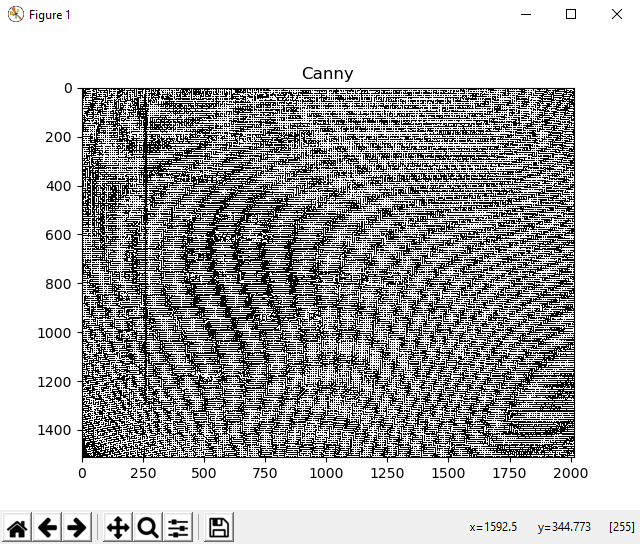
\includegraphics[width=10cm]{img/canny_error.png}
\caption{Lỗi khi áp dụng Canny nhưng không lọc nhiễu, áp dụng với ảnh src201.jpeg}
\end{figure}

Bên cạnh đó, mỗi loại hình ảnh cần các giá trị min\_threshold và max\_threshold khác nhau khi áp dụng Canny:

\begin{itemize}
	\item Ảnh loại (1): min\_threshold = 50, max\_threshold = 200
	\item Ảnh loại (2): min\_threshold = 10, max\_threshold = 15
\end{itemize}

\subsection{Source code sử dụng các thư viện OCR}

\subsubsection{Sử dụng thư viện pytesseract}

\lstinputlisting[language=Python, linerange={24-33}]{ocr.py}

\subsubsection{Sử dụng thư viện pyocr}

\lstinputlisting[language=Python, linerange={34-50}]{ocr.py}

\subsubsection{Sử dụng thư viện tesserocr}

\lstinputlisting[language=Python, linerange={53-56}]{ocr.py}

\subsubsection{So sánh mức độ trùng nhau giữa 2 đoạn text}

Sử dụng thư viện difflib được hỗ trợ sẵn bởi ngôn ngữ Python:

\lstinputlisting[language=Python, linerange={166-179}]{main.py}

\subsubsection{Thu thập kết quả chạy của source code OCR với từng test case}

\lstinputlisting[language=Python, linerange={18-21}]{ocr.py}

\begin{lstlisting}[language=Python]
def summary(max_img_id):
    overall = {"pytesseract": [], "pyocr": [], "tesserocr": []}
    for img_id in range(1, max_img_id+1):
        if get_image_filename(img_id) is not None:
           for libname in ["pytesseract", "pyocr", "tesserocr"]:
               ratio = compare_output(libname, img_id)
               print(img_id, libname, round(ratio*100, 2))
               overall[libname].append(ratio)

    print("OVERALL")
    for libname in ["pytesseract", "pyocr", "tesserocr"]:
        s = sum(overall[libname])
        n = len(overall[libname])
        print(libname, round(100*s/n, 2))
\end{lstlisting}

\section{Đánh giá kết quả}

Bảng dưới đây ghi lại mức độ giống nhau của kết quả thu được sau quá trình OCR với output mẫu khi không cắt ảnh và chỉ thực hiện lọc nhiễu ảnh của 1 số mẫu.

\begin{tabular}{|c|c|c|c|}
\hline & \multicolumn{3}{c|}{Thư viện} \\
\hline \textbf{Mã số} & \textbf{pytesseract} & \textbf{pyocr} & \textbf{tesserocr} \\
\hline \textbf{001} & 65.33\% & 65.44\% & 65.39\% \\
\hline \textbf{003} & 76.14\% & 75.35\% & 75.28\% \\
\hline \textbf{004} & 45.26\% & 45.45\% & 45.66\% \\
\hline \textbf{005} & 75.24\% & 77.67\% & 74.53\% \\
\hline \textbf{006} & 31.01\% & 29.79\% & 43.09\% \\
\hline \textbf{007} & 74.14\% & 71.55\% & 71.25\% \\
\hline \textbf{Tổng hợp} & 61.21\% & 60.87\% & 62.63\% \\
\hline
\end{tabular}

(Bảng đầy đủ được ghi ở file báo cáo riêng)

\noindent Một số kết luận khác ta có thể rút ra được:

\begin{itemize}
	\item Trên hệ điều hành Windows, thư viện pytesseract chạy rất chậm trên ảnh jpeg.
	\item Ảnh dark theme chạy ít chính xác hơn ảnh light theme.
	\item 1 số ảnh không detect được: 90, 97, 104, 105, 106, 107, 108.
\end{itemize}

\section{Kết luận}

\indent Trong số 3 thư viện trên, ta có thể sử dụng thư viện tesserocr vì độ chính xác tốt nhất, mặc dù độ chính xác chưa thực sự cao. Ta chưa xét đến yếu tố thời gian, vì thời gian chạy của mỗi thư viện phụ thuộc vào hệ điều hành và định dạng ảnh đưa vào.

Công việc tốn thời gian nhất là cắt ảnh. Hough Transform phát hiện đường thẳng khá tốt, nhưng lựa chọn dựa vào đường thẳng nào để cắt là một bài toán rất khó. Nếu ta cắt ảnh vừa đúng, kết quả của quá trình OCR sẽ chính xác hơn.

Toàn bộ font chữ của các ảnh đầu vào đều là monospace, tập kí tự khác nhau khá giới hạn, các kí tự có độ rộng bằng nhau. Tuy nhiên trái với suy nghĩ ban đầu của tác giả, bài toán nhận dạng đã trở nên khó. Trong các yếu tố ảnh hưởng đến kết quả của quá trình OCR, độ tương phản, kích thước và chất lượng của ảnh, độ lớn của chữ là 4 yếu tố đầu tiên. Tập ảnh thu thập từ các nguồn trong thực tế, không đảm bảo tốt 4 yếu tố trên nên kết quả có sự sai lệch nhiều.

Project này tiếp cận bài toán theo xử lý ảnh, chỉ sử dụng các kỹ thuật cơ bản của xử lý ảnh và chưa sử dụng các công nghệ cao cấp hơn. Thay vì giải quyết một cách bán tự động như code trong project này, một giải pháp tự động hơn sẽ làm tăng hiệu quả giải quyết bài toán. Ví dụ:

\begin{itemize}
	\item Học cách nhận diện đường cần cắt theo màu sắc và độ dày.
	\item Dựa vào độ rộng của 1 số kí tự, tính khoảng cách từ đầu dòng đến lề để tính số dấu cách đầu dòng cần thiết.
\end{itemize}

Trong tương lai, nếu áp dụng Deep Learning vào OCR, chất lượng của các OCR engine sẽ được cải thiện mà có thể bỏ qua các yếu tố về ảnh (độ tương phản, kích thước, chất lượng của ảnh và kích thước của chữ).

\section{Tài liệu tham khảo}

\begin{itemize}
	\item \textit{Awesome OCR}. \url{https://github.com/kba/awesome-ocr\#python}
	\item AnandhJagadeesan (2020, February 19). \textit{Text Detection and Extraction using OpenCV and OCR}. GeeksforGeeks. \url{https://www.geeksforgeeks.org/text-detection-and-extraction-using-opencv-and-ocr}
	\item Tim Chin (2019, January 23). \textit{Using Image Processing to Detect Text}. Medium. \url{https://medium.com/@theclassytim/using-image-processing-to-detect-text-8be34c677c11}
	\item \textit{Image denoising by FFT.} \url{http://scipy-lectures.org/intro/scipy/auto_examples/solutions/plot_fft_image_denoise.html}
	\item \textit{7 Tips to Improve OCR Accuracy (Why is my OCR so poor?)}. YouTube. \url{https://www.youtube.com/watch?v=KS1gd5yUmKo}
\end{itemize}

\end{document}